\chapter{(Network) Flow Problems}

\begin{descr}
    TODO
\end{descr}

\section{Network Flow Problems}\index{Network Flow Problems}
\begin{example}
Example: Oil field + transportation

\end{example}

\begin{definition}
A network N consists of 
\begin{enumerate}
\item A finite directed graph $G=(V,E)$ without loops and parallel edges
\item a function $c: E -> \mathds{R}^{+}$, which assigns a capacity to each edge
\item two designated nodes s and t, called \deftxt{source} and \deftxt{sink}
\end{enumerate}
Short: $N = (G, c, \{s, t\})$
\end{definition}

\begin{definition}
Let $N = (G, c, \{s, t\})$ be a network. A flow function on N is a function $f: E -> \mathds{R}$ such that 
\begin{itemize}
\item $ 0 \le f(e) \le c(e), \forall e \in E $
\item $ \alpha(v) := \{e:$ endpoint of e is v $\}, v \in V$ \\
$\beta(v) := \{e:$ startpoint of e is v $\}, v \in V$
\end{itemize}
For every $v \in V\backslash\{s, t\} $ \\
$ \sum_{e \in \alpha(v)} f(e) = \sum_{e \in \beta(v)} f(e) $ \\
This is called \deftxt{"conservation function"}. \\
The \deftxt{total flow} of the flow function is given by $F = \sum_{e \in \alpha(t)} f(e) - \sum_{e \in \beta(t)} f(e) $
\end{definition}

\begin{example}
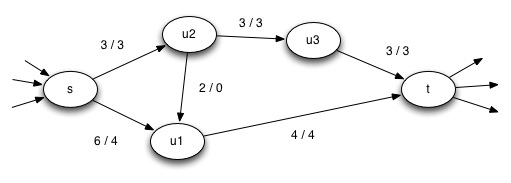
\includegraphics{diagrams/Chapter3_Example1.jpg}
\\Notion: $ 6 / 4 $ describes the capacity and the flow of an edge. In this example the capacity of the edge is 6 and the flow is 4.
\end{example}

Problem: \\
Given an arbitrary network N, find a flow function f, where the total flow F is maximal. \\

\begin{definition}
Let N = $(G, c, \{s, t\})$ be a network. Let $S \subseteq V$ with s $\in S, t \notin S$ \\
$\bar{S} = V \backslash S$ (i.e. $t \in \bar{S}$) \\
$E_{S\bar{S}} = \{e:$ all edges with starting point in S and endpoint in $\bar{S} \}$ \\
$E_{\bar{S}S} = \{e:$ all edges with start point in $\bar{S}$ and end point in S $\}$ \\
$E_{S\bar{S}} \cup E_{\bar{S}S} $ is the \deftxt{cut} defined by S. \\
The capacity of a cut defined by S: $c(S) = \sum_{e \in E_{\bar{S}S}}c(e)$
\end{definition}

\begin{lemma}
Let $N =(G, c, \{s, t\})$ be a network, $f: E \rightarrow \mathds{R}$ be a flow function then for any $S \subseteq V$ with $s \in S, t \notin S$: 
\[
F = \sum_{e \in E_{S\bar{S}}}f(e) - \sum_{e \in E_{\bar{S}S}} f(e)
\]
\end{lemma}

\begin{proof}
\[ F = \sum_{e \in \alpha(t)} f(e) - \sum_{e_ \in \beta(t)} f(e) \]
\[0 = \sum_{e \in \alpha(v)} f(e) - \sum_{e \in \beta(v)} f(e); \forall v \in \bar{S} \backslash \{t\} \]
We add all these equations up. Left hand side: $F$ remains. Right hand side: Let $x \xrightarrow{e} y$ be an edge. We need to consider 4 cases:
\begin{enumerate}
\item $x, y \in S$, then the value $f(e)$ does not occur in the summation
\item $x, y \in \bar{S}$, then $f(e)$ occurs one time positive in the summation, namely for y \\ f(e) occurs one time negative in the summation, namely for x 
\item $x \in S; y \in \bar{S}$, f(e) occurs positive for y and nowhere else and $e \in E_{S\bar{S}}$
\item $x \in \bar{S}; y \in S$, then $f(e)$ occurs negative for x and nowhere else and $e \in E_{\bar{S}S}$
\end{enumerate}
This leads to the following equation:
\[F = \sum_{e \in E_{S\bar{S}}}f(e) - \sum_{e \in E_{\bar{S}S}} f(e) \]
Only case 3 are 4 contribute.
\end{proof}

\begin{lemma}
For every flow function f with total flow F and any ser $S \subseteq V$, $s \in S$, $t \notin S$
$$ F \le c(S) $$
\end{lemma}

\begin{proof}
From lemma 3.1 we know
\[F = \sum_{e \in E_{S\bar{S}}}f(e) - \sum_{e \in E_{\bar{S}S}}f(e) \le \sum_{e \in E_{S\bar{S}}}f(e) \le \sum_{e \in E_{S\bar{S}}}c(e) = c(S) \] 
\end{proof}

\begin{corollary}[Max Flow - Min Cut Statement]
If $F=c(S)$ then the total flow F is \underline{maximal} and the capacity of the cut defined by $S$ is \underline{minimal}.
\end{corollary}

\begin{proof}
Let $F = c(S)$, consider another flow function $f'$ with total flow $F'$.
\begin{enumerate}
\item $F' \le c(S)$ (Lemma 3.2) // $F' \le c(S) = F$ \\Hence, f is a flow function with maximal total flow.
\item Let $S'$ with $s \in S'$, $t \notin S'$ be given. $c(S) = F \le c(S')$. Hence the capacity $c(S)$ is minimal among all other capacities. 
\end{enumerate}
\end{proof}

An \deftxt{augmenting path} is a simple path from s to t, that is not necessarily directed. And for which the following two cases hold: Let e be an edge on this path: 
\begin{enumerate}
\item $ s \rightarrow \circ \rightarrow \circ \rightarrow ... \rightarrow \underset{s_i}{\circ} \xrightarrow{e} \underset{s_{i+1}}{\circ} ...  \underset{t}{\circ}$ then we request that $f(e) < c(e)$
\item $s \rightarrow \circ ...  \underset{s_i}{\circ} \xleftarrow{e} \underset{s_{i+1}}{\circ} ... \underset{t}{\circ}$ then we request that $f(e) > 0$
\end{enumerate}

\begin{example}
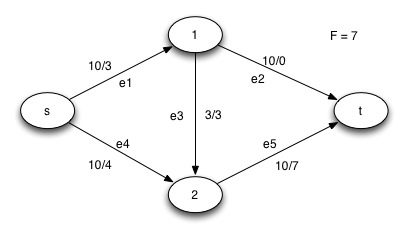
\includegraphics{diagrams/Chapter3_Example2.jpg} \\
Which of the following is an augmenting path? 
\begin{itemize}
\item $e_1 e_2$
\item $e_1 e_3 e_5$
\item $e_4 e_3 e_2$
\item $e_4 e_5$
\end{itemize}

Solution: \\
The first, third and fourth example are augmenting paths. The second path violates case 1.
\end{example}

We use $e_4 e_3 e_2$ to improve the flow function as follows:
\begin{itemize}
\item For forward egdes $e: c(e) - f(e)$:
\begin{itemize}
	\item $e_4: 6$
	\item $e_2: 10$
\end{itemize}
\item For backward edges $e: f(e)$
\begin{itemize}
\item $e_3: 3$
\end{itemize}
\end{itemize}
We chose the minimum from the values and add the value to the flow of forward egdes and substract it from backward egdes. The flows of the edges change as follows:
\begin{itemize}
\item $e_4  \xfrac{10}{7}$
\item $e_2 \xfrac{10}{3}$
\item $e_3 \xfrac{3}{0}$
\end{itemize} 

\begin{example}
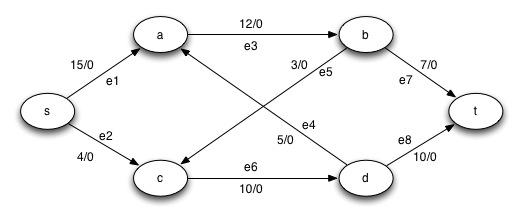
\includegraphics{diagrams/Chapter3_Example3.jpg} \\
Augmenting path: \\
$s* \xrightarrow{e_2} c* \xrightarrow{e_6} d* \xrightarrow{e_4} a* \xrightarrow{e_3} b* \xrightarrow{e_7} t*$ \\
Compute deltas:
\begin{itemize}
\item $\Delta_{(e_2)} = 4$
\item $\Delta_{(e_6)} = 10$
\item $\Delta_{(e_4)} = 5$
\item $\Delta_{(e_3)} = 12$
\item $\Delta_{(e_7)} = 7$
\end{itemize}
The minimum $\Delta$ is 4, so the flow of the edges will be increased by 4.
\begin{itemize}
\item $e_2 = \xfrac{4}{4}$
\item $e_6 = \xfrac{10}{4}$
\item $e_4 = \xfrac{5}{4}$
\item $e_3 = \xfrac{12}{4}$
\item $e_7 = \xfrac{7}{4}$
\end{itemize} 

The next steps or paths would be:
\begin{itemize}
\item $s \rightarrow a \rightarrow b \rightarrow c \rightarrow d \rightarrow t$
\item $s \rightarrow a \rightarrow b \rightarrow t$
\item $s \rightarrow a \rightarrow d \rightarrow t$
\end{itemize}
The application of this paths leads to a new flow: $F = 14$.
\end{example}

\begin{lemma}
When executing a step in the algorithm, the actual function f is a flow function.
\end{lemma}

\begin{proof}
The assumption is obviously true for step 1 because $f \equiv 0$ is a flow function. It is obviously true for steps 2, 3 and 5, too, because f is not modified. \\
Step 4: \\
Let $f$ be a flow function when we enter step 4. We have to show that after performing step 4, the newly calculated function $f$ is still a flow function. \\
Let $f_{old}$ be the function with which we enter step 4 and $f_{new}$ the newly calculated one. $f_{old}$ is a flow function. Hence, 
\[
\]
\end{proof}